\chapter{Distributed Delay Model}\label{section:distdel}

A systematic study of distributed delay in the context of Turing instabilities is extremely sparse in current literature, with no work having been previously done looking at the Schnakenberg model. In this chapter, we consider the LI model with time delay modelled as a (skewed) truncated Guassian distribution. The quadrature rule we use to produce numerical simulations is first considered. The linear analysis conducted for the fixed delay case is then extended to the distributed delay model, and we look to show analytically that a symmetric truncated Gaussian distribution does not have a qualitative difference on the results seen, and thus does not resolve some of the key problems highlighted in the fixed delay case. These results are also verified through numerical simulations.

\section{Composite Simpson's Rule}\label{section:quad}

The LI model with distributed time delay, as defined in \eqref{distmodel}, is given as

\begin{equation}\label{distmodel2}
  \begin{split}
    \frac{\partial u}{\partial t}&=\frac{\epsilon^2}{L^2}\frac{\partial^2u}{\partial x^2}+a-u-2u^2v+3\int_{a}^{b}k(s,\textbf{p})\hat{u}^2\hat{v} \ \text{ds},\\
    \frac{\partial v}{\partial t}&=\frac{1}{L^2}\frac{\partial^2v}{\partial x^2}+b-u^2v,
\end{split}
\end{equation}
where $\hat{u}=u(x,t-s)$ and $\hat{v}=v(x,t-s)$ where $s$ is the integration variable ranging over the delays. The integration domain $[a, b]$, can be discretised into $N$ sub-intervals of equal length with $N+1$ discretisation points, $s_0,\cdots,s_{N}$, such that $s_0=\tau-n\sigma$ and $s_N=\tau+n\sigma$. Using the composite Simpsons's rule \cite{compsimp}, the integral term can be numerically approximated as

\begin{equation}\label{simp}\int_{a}^{b}k(s)\hat{u}^2\hat{v}\  \text{ds}\approx\frac{h}{3}\left[k(s_0)\hat{u}^2_0\hat{v}_0+2\sum_{i=1}^{\frac{N}{2}-1}k(s_{2i})\hat{u}^2_{2i}\hat{v}_{2i}+4\sum_{i=2}^{\frac{N}{2}}k(s_{2i-1})\hat{u}^2_{2i-1}\hat{v}_{2i-1}+k(s_N)\hat{u}^2_N\hat{v}_N\right],
\end{equation}
where $h$ is computed as $h=\frac{b-a}{N}$. We use the notation $\hat{u}_j$ and $\hat{v}_j$ to denote $u(t-s_j)$ and $v(t-s_j$) respectively, namely the functions $u$ and $v$ evaluated at time-delay with some index $j$, $s_j$.

\section{A Symmetric Distribution}\label{section:symmetric}
\subsection{Introduction}

As done in \cite{william}, by assuming each individual mechanism within the gene expression process acts independently and identically, we use the central limit theorem to model the delay as a (skewed) Gaussian distribution with parameters $\textbf{p}=(\tau,\sigma)$, for some mean $\tau$ and standard deviation $\sigma$. We begin by using a symmetric truncated distribution with integration limits $a=\tau-n\sigma$ and $b=\tau+n\sigma$ for some $n\in\mathbb{N}$, such that $a=\tau-n\sigma>0$. We can thus write the LI model with distributed time delay as

\begin{equation}\label{symmod}
    \begin{split}
        \frac{\partial u}{\partial t}&=\frac{\epsilon^2}{L^2}\frac{\partial^u}{\partial x^2}+a-u-2u^2v+3\int_{\tau-n\sigma}^{\tau+n\sigma}k(s;\tau,\sigma)\hat{u}^2\hat{v}\ \text{ds},\\
        \frac{\partial v}{\partial t}&=\frac{1}{L^2}\frac{\partial^2v}{\partial x^2}+b-u^2,
    \end{split}
\end{equation}
where $\hat{u}=u(x,t-s)$ and $\hat{v}=v(x,t-s)$, with $s$ the integration variable ranging over the delays. The function $k(s;\tau,\sigma)$ is the symmetric truncated Gaussian pdf given by \cite{cite}

\begin{equation}
k(s;\tau,\sigma)=\Phi_cf\left(\frac{s-\tau}{\sigma}\right).
\end{equation}
with $f(x)$ the general pdf of the Gaussian distribution given as
\begin{equation}\label{f}
    f(x)=\frac{1}{\sqrt{2\pi}\sigma}\exp\left(-\frac{1}{2}x^2\right).
\end{equation}
We use $\Phi_c$ to denote the truncated scaling constant. This constant ensures that $k(s;\tau,\sigma)$ integrates to $1$ over the given integration domain $[a,b]$, and is computed as
\begin{equation}
    \Phi_c=\frac{1}{\phi\left(\frac{b-\tau}{\sigma}\right)-\phi\left(\frac{a-\tau}{\sigma}\right)},
\end{equation}
with $\phi(x)$ the cdf of the Gaussian distribution. This is given by
\begin{equation}\label{phi}
    \phi(x)=\frac{1}{2}\left(1+\text{erf}\left(\frac{x}{\sqrt{2}}\right)\right).
\end{equation}

Throughout this section we use $n=3$ so that the integration limits are $a=\tau-3\sigma$ and $b=\tau+3\sigma$. This was chosen so that a relatively large $\sigma$ value could be chosen for each $\tau$ while maintaining $a>0$. For each $\tau$ value, a maximum $\sigma$ value can be computed such that $a=\tau-3\sigma\geq0$ as $\sigma_{\max}=\frac{\tau}{3}$. By setting $\sigma<\sigma_{\max}$, we ensure that the integration domain strictly considers positive time delays only.

Figures \ref{fig:pdf1} and \ref{fig:pdf2} show the pdf of a truncated Gaussian distribution centred at a mean $\tau=1,2$ with varying $\sigma$ values as fractions of $\sigma_{max}$. We have $s$ as the integration variable, with $s\in[a,b]$.

\begin{figure}[H]
    \centering
    \begin{subfigure}[b]{0.45\textwidth}
        \centering
        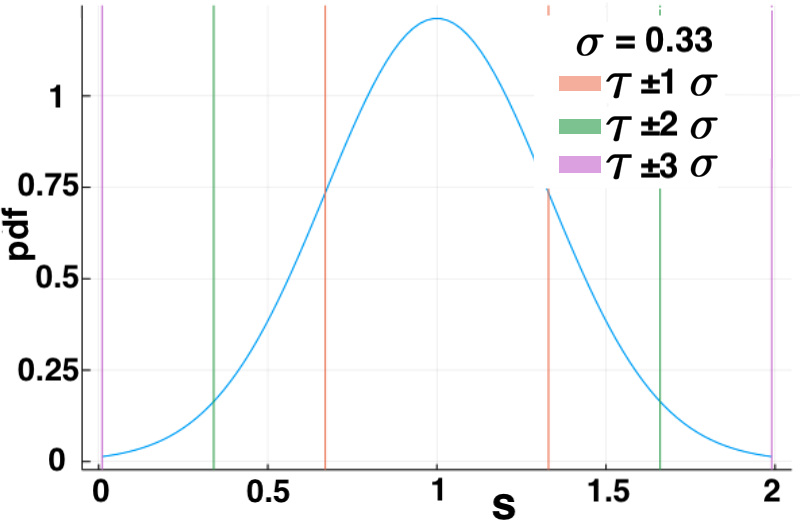
\includegraphics[width=7cm,height=5cm]{t1sig1.png}
        \caption{Truncated Gaussian distribution following $\mathcal{N}(1,(\sigma_{max}\times0.99)^2)$}
        \label{}
    \end{subfigure}
    \hfill
    \begin{subfigure}[b]{0.45\textwidth}
        \centering
        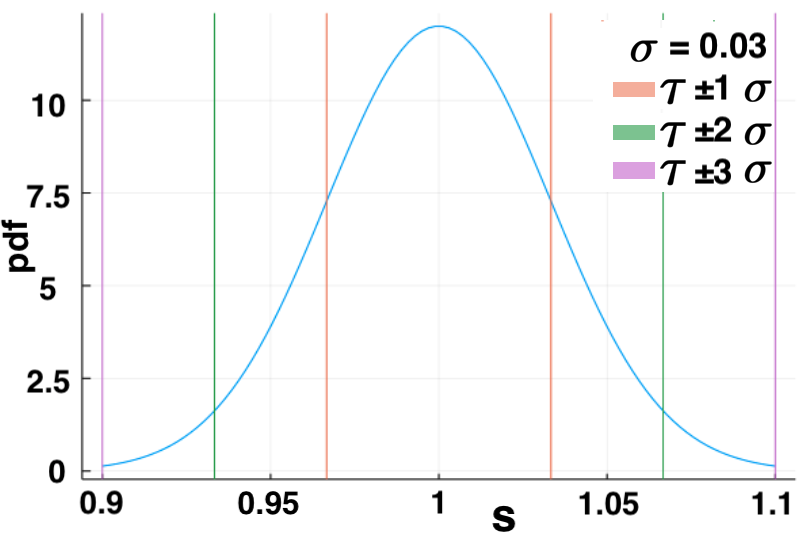
\includegraphics[width=7cm,height=5cm]{t1sig2.png}
        \caption{Truncated Gaussian distribution following $\mathcal{N}(1,(\sigma_{max}\times0.1)^2)$}
        \label{}
    \end{subfigure}
\caption{PDF of truncated Gaussian distribution with mean $\tau=1$ and integration domain $[1-3\sigma,1+3\sigma]$. $\sigma$ values of $0.33(2.d.p)$ and $0.03(2.d.p)$ are considered.}
\label{fig:pdf1}
\end{figure}
\begin{figure}[H]
    \centering
    \begin{subfigure}[b]{0.45\textwidth}
        \centering
        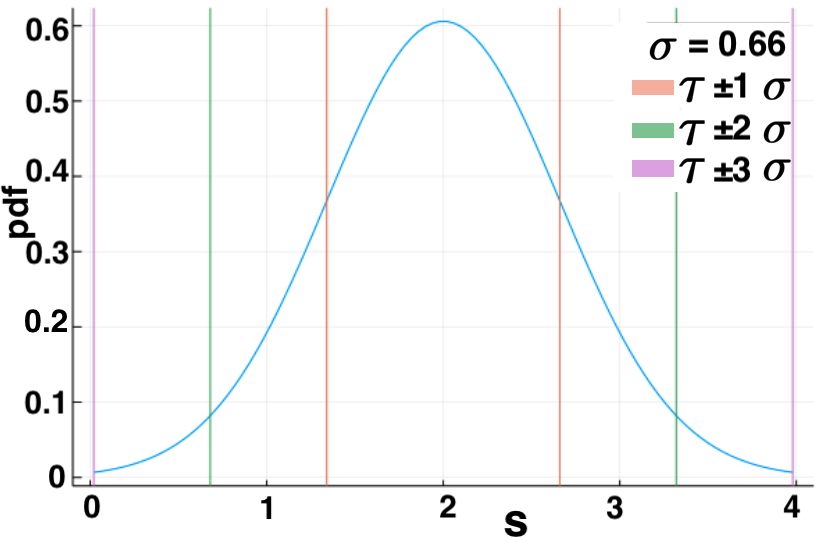
\includegraphics[width=7cm,height=5cm]{t2sig1.png}
        \caption{Truncated Gaussian distribution following $\mathcal{N}(2,(\sigma_{max}\times0.99)^2)$}
        \label{}
    \end{subfigure}
    \hfill
    \begin{subfigure}[b]{0.45\textwidth}
        \centering
        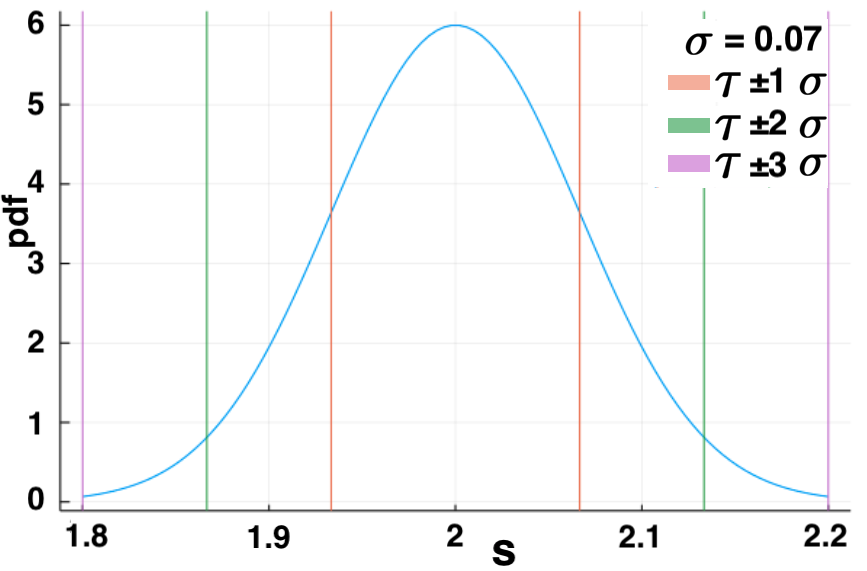
\includegraphics[width=7cm,height=5cm]{t2sig2.png}
        \caption{Truncated Gaussian distribution following $\mathcal{N}(2,(\sigma_{max}\times0.1)^2)$}
        \label{}
    \end{subfigure}
    \caption{PDF of truncated Gaussian distribution with mean $\tau=2$ and integration domain $[2-3\sigma,2+3\sigma]$. $\sigma$ values of $0.66(2.d.p)$ and $0.07(2.d.p)$ are considered.}
    \label{fig:pdf2}
\end{figure}
We see that $\sigma$ is responsible for scaling on the $x$-axis, while the truncation constant $\Phi_c$, defined in \eqref{distmodel}, scales the $y$-axis, ensuring the pdf integrates to $1$ across the integration domain. For the implementation of the quadrature rule, the number of sub-intervals $N$ was chosen to qbe $N=50$. The consideration for such a choice involves both quadrature accuracy and computational efficiency. In this section, we present results obtained in testing the quadrature rule, to show that $N=50$ is a sufficiently large choice. We apply the quadrature to two test integrals: the first is the truncated Gaussian pdf $k(s,\tau,\sigma)$, which should analytically integrate to $1$. For the second test, we apply the quadrature rule to both a spatially and temporally dependent integral, which can be evaluated analytically, given by
\begin{equation}\label{testint}
\int_a^bk(s,\tau,\sigma)f(x,t-s)\ \text{ds},
\end{equation}
where $f(x,t)=xt$. This can be explicitly evaluated as

\begin{equation}
    \begin{split}
&\int_a^bk(s,\tau,\sigma)f(x,t-s)\ \text{ds}=xt\int_a^bk(s,\tau,\sigma)\ \text{ds}-x\int_a^bk(s,\tau,\sigma)s\ \text{ds}\\&=xt\left[\frac{\Phi_c}{2}\text{erf}\left(\frac{s-\tau}{\sqrt{2}\sigma}\right)\right]\bigg|_a^b-x\left[\frac{\Phi_c}{2}\text{erf}\left(\frac{s-\tau}{\sqrt{2}\sigma}\right)-\frac{\Phi_c\sigma}{\sqrt{2\pi}}\exp\left(-\frac{1}{2}\left(\frac{s-\tau}{\sigma}\right)^2 \right)\right]\Bigg|_a^b.
    \end{split}
\end{equation}

Figures in appendix \ref{section:appB} show the relative (and absolute error) of the quadrature rule applied to the truncated Guassian pdf $k(s,\tau,\sigma)$ for different $N$, with a fixed $\tau=1$ and $\sigma=\sigma_{max}\times0.1$. We only consider a fixed $\tau$ and $\sigma$ here, as further numerical solutions in appendix \ref{section:appB} for varying $\tau$ values show that the relative error results are independent of $\tau$ and $\sigma$. Results in appendix \ref{section:appB} also show the relative error of the quadrature rule applied to \eqref{testint} for $t\in[1.1,500]$ and $x\in[0.1,1]$, for a fixed $\tau=1$ and $\sigma=\sigma_{max}\times0.1$, and $N=50$. The spatial and temporal domains were chosen to discard the effects of catastrophic cancellation, which is caused by very small solution values for $0\leq t\leq 1.1$ and $0\leq x\leq 0.1$. The results show that the relative error (in absolute value) of the composite Simpson's rule applied to both test integrals, with $N=50$, is of $O(10^{-4})$, namely $<0.1\%$ error, independent of $\tau$ and $\sigma$, across both spatial and temporal domains. We therefore conclude that using $N=50$ quadrature points is sufficiently large.


\subsection{Linear Analysis}\label{section:distlin}
Taking a small perturbation about the steady-state $u=u_\star+\delta\xi$, $v=v_\star+\delta\eta$, where $|\delta|\ll1$, we can write the equation for the activator $u$ in \eqref{distmodel2} as

\begin{equation}\label{perturb}
  \delta\frac{\partial \xi}{\partial t}=\delta \frac{\epsilon^2}{L^2}\frac{\partial^2\xi}{\partial x^2}+f(u_\star+\delta\xi, v_\star+\delta\eta)+g(u_\star+\delta\hat{\xi},v_\star+\delta\hat{\eta}) ,
\end{equation}
where $f(u,v)=a-u+2u^2v$ and $g(\hat{u},\hat{v})=3\int_a^bk(s)\hat{u}^2\hat{v} \text{ds}$. The $\hat{\xi}$ notation is used to denote the perturbation evaluated at a delay $\hat{\xi}=\xi(x,t-s)$. Taylor expanding equation \eqref{perturb} for the $f$ term about the steady-state and evaluating the $g$ term, up to $O(\delta)$, yields

\begin{dmath}\label{taylor}
  \delta\frac{\partial \xi}{\partial t}=\delta \frac{\epsilon^2}{L^2}\frac{\partial^2\xi}{\partial x^2}+f(u_\star,v_\star)+3u_\star^2v_\star\int_a^bk(s)\text{ds}+\delta\left[\xi f_u(u_\star,v_\star)+\eta f_v(u_\star,v_\star)+6u_\star v_\star\int_a^bk(s)\hat{\xi}\text{ds}+3u_\star^2\int_a^bk(s)\hat{\eta}\text{ds}
  \right].
\end{dmath}
We use the notation $f_u$ to denote the derivative of function $f$ with respect $u$. Using the facts that the truncated Guassian $k(s)$ integrates to $1$ over $[a,b]$, and evaluation the expressions $f_u(u_\star,v_\star)$ and $f_v(u_\star,v_\star)$, equation \eqref{taylor} can be simplified to

\begin{equation}\label{linu}
  \delta \frac{\partial \xi}{\partial t}=\delta \frac{\epsilon^2}{L^2}\frac{\partial^2\xi}{\partial x^2}+\delta\left[\xi(-1-4u_\star v_\star)-2\eta u_\star^2 +6u_\star v_\star\int_a^bk(s)\hat{\xi}\text{ds}+3u_\star^2\int_a^bk(s)\hat{\eta}\text{ds}\right].
\end{equation}
The linearised dynmacs for $v$ are more simply given by
\begin{equation}\label{linv}
\delta \frac{\partial\eta}{\partial t}=\delta \frac{1}{L^2}\frac{\partial^2\eta}{\partial x^2}-\delta\left[2\xi u_\star v_\star+\eta u_\star^2\right].
\end{equation}
Dividing through by $\delta$ and substituting in an ansatz of the form $\xi=\xi_0e^{\lambda_k t}\cos(k\pi x)$ \cite{yigaffneyli} into \eqref{linu} and $\eta=\eta_0e^{\lambda_k t}\cos(k\pi x)$ into \eqref{linv}, and then dividing through by $e^{\lambda_k t}$ and $\cos(k\pi x)$, results in

\begin{equation}\label{sysof}
  \begin{split}
\lambda_k\xi_0&=-\frac{\epsilon^2}{L^2}k^2\pi^2\xi_0+\xi_0(-1-4u_\star v_\star)-2\eta_0u_\star^2+6\xi_0u_\star v_\star E+3\xi_0u_\star^2E \\
\lambda_k\eta_0&=-\frac{1}{L^2}k^2\pi^2\eta_0-2\xi_0u_\star v_\star-\eta_0u_\star^2,
\end{split}
\end{equation}
where $E=\int_a^bk(s,\tau,\sigma)e^{-\lambda_k s}\text{d}s$. We can write equation \eqref{sysof} as a homogeneous linear system for $(\xi_0,\eta_0)^T$, given by

\begin{equation}
\underbrace{\begin{pmatrix}-1-4u_\star v_\star-\frac{\epsilon^2}{L^2}k^2\pi^2+6u_\star v_\star E-\lambda_k&-2u_\star^2+3u_\star^2E\\-2u_\star v_\star&-u_\star^2-\frac{1}{L^2}k^2\pi^2-\lambda_k \end{pmatrix}}_{\textbf{M}}\begin{pmatrix}\xi_0\\\eta_0\end{pmatrix}=\begin{pmatrix}0\\0\end{pmatrix}.
\end{equation}
Looking for non-trivial solutions, we look for roots of the characteristic equation, namely $D_k=\text{det}(\textbf{M})=0$. The characteristic equation, $D_k$, is given as
\begin{equation}\label{characdist}
  D_k=\lambda_k^2+\alpha_k\lambda_k+\beta_k+(\gamma_k\lambda_k+\delta_k)E=0,
\end{equation}
where
\begin{align}
\alpha_k&=\left(\frac{\epsilon^2}{L^2}+\frac{1}{L^2}\right)k^2\pi^2+u_\star^2+4u_\star v_\star+1\\
\beta_k&=\left(\frac{1}{L^2}\pi^2k^2+u_\star^2\right)\left(\frac{\epsilon^2}{L^2}\pi^2k^2+4u_\star v_\star+1\right)-4u_\star^3v_\star\\
\gamma_k&=-6u_\star v_\star\\
\delta_k&=-\frac{6}{L^2}u_\star v_\star k^2\pi^2.
\end{align}

Finally, we note that the expression $E$ can be evaluated as
\begin{equation}
E=\int_a^bk(s,\tau,\sigma)e^{-\lambda_k s}\ \text{d}s=\frac{\Phi_c}{2}\left[\exp\left(\frac{\lambda_k(\lambda_k\sigma^2-2\tau)}{2}\right) \text{erf} \left(\frac{\lambda_k\sigma^2+s-\tau}{\sqrt{2}\sigma}\right)\right]\Bigg|_a^b.
\end{equation}
The charactersitic equation \eqref{characdist} cannot trivially be split into it's real and imaginary components due to the error function term in $E$ as was done in the fixed delay case. We therefore cannot explicitly compute the stability lines in $(a,b)$ parameter space. We can however range over $(a,b)$ and compute $\max_k(\Re(\lambda_k))$ for different $\tau$, and produce plots similar to those in figures \ref{fig:dispfixed} and \ref{fig:lambdavary}. We use these plots to pseudo-analytically prove that, using a symmetric Gaussian distribution centred at mean $\tau$ will not change the time-to-pattern seen for a fixed delay of $\tau$, independent of the standard deviation of the distribution $\sigma$. We first plot $\max_k(\Re(\lambda_k))$ against $\tau$, as seen analogously in figure \ref{fig:dispfixed} for the fixed delay case, for multiple parameters $(a,b,\tau,\sigma)$, and compares these to the fixed delay case. Since physically we cannot have negative delays, we require the lower integration limit to be positive. Namely, for a given mean $\tau$, we require $\tau-3\sigma>0$. We therefore define a maximum $\sigma$ value by $\sigma_{max}=\tau / 3$. By ensuring $\sigma<\sigma_{max}$, we ensure only positive delays are considered.

Figures \ref{fig:p2} and \ref{fig:p3} show $\max_k(\Re(\lambda_k))$ plotted against $\tau\in[0,1]$ for two different parameter sets $(a,b)=\{(0.1,0.9), (0.4,0.4)\}$, for the fixed delay case. For each parameter set, figures are produced with different $\sigma$ values as a fraction of $\sigma_{max}$, and the absolute value of the difference between $\max_k(\Re(\lambda_k))$ for each distributed delay case compared with the fixed delay case is plotted. We note that in the distributed delay case, as we vary $\tau$, $\sigma_{max}$ and thus the integration limits both change as functions of $\tau$. All numerical results in this chapter are produced with $L=30\sqrt{0.05}$, and unless otherwise stated, $\epsilon^2=0.001$.

% PARAMTER SET 2
\begin{figure}[H]
    \centering
    \begin{subfigure}[b]{0.45\textwidth}
        \centering
        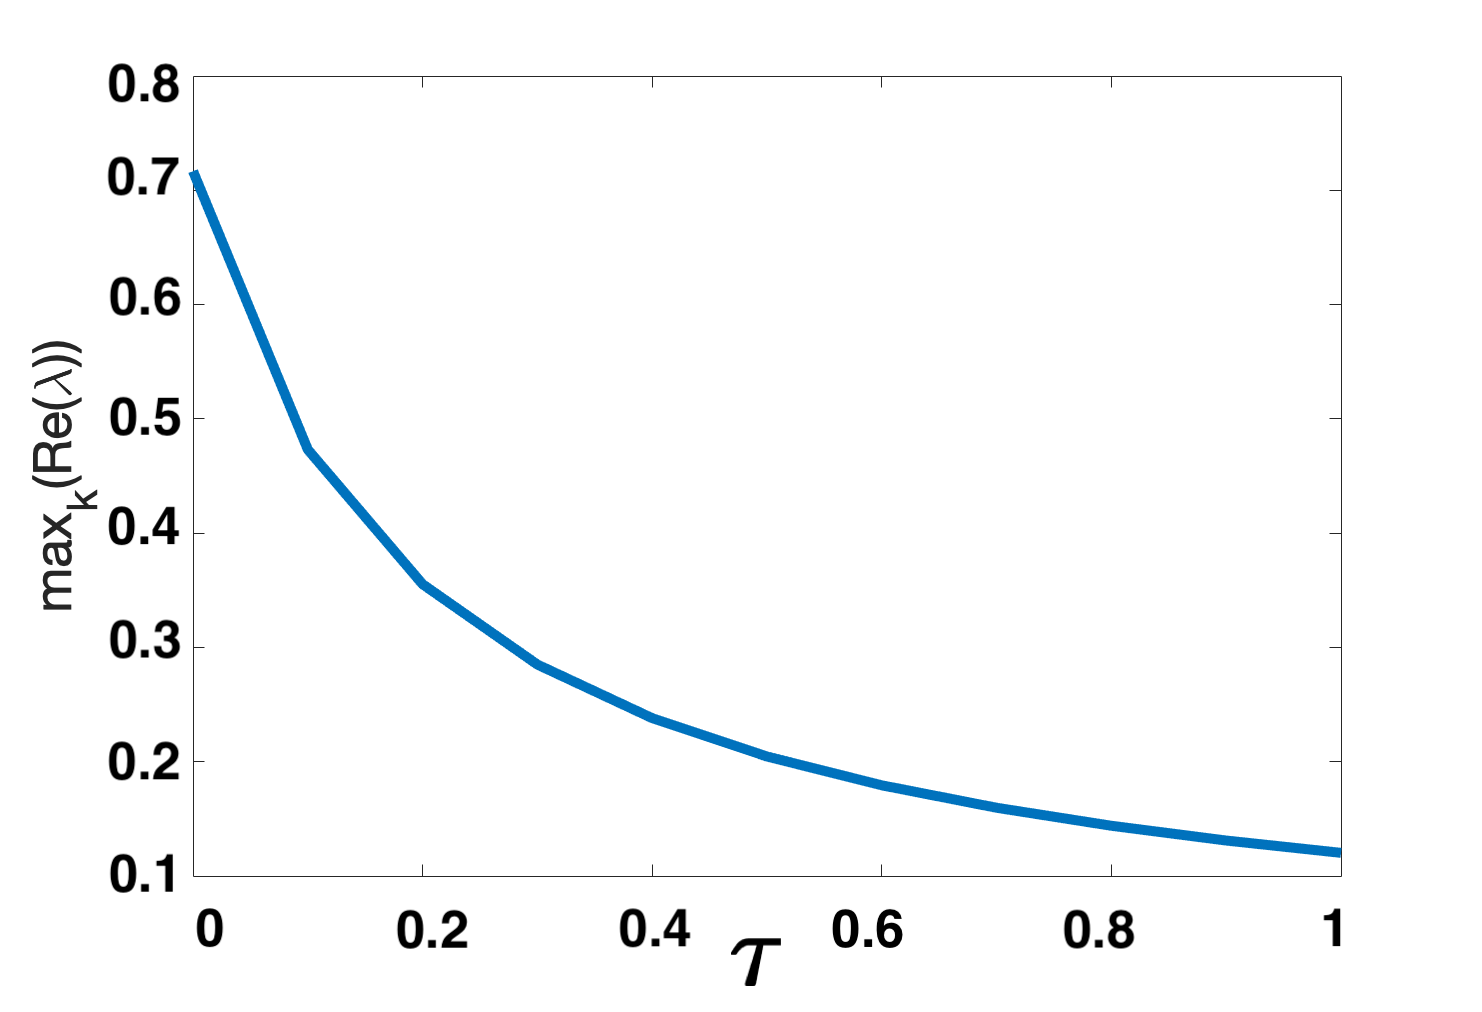
\includegraphics[width=7cm,height=5cm]{p2fixed.png}
        \caption{Fixed delay case.}
        \label{}
    \end{subfigure}
    \hfill
    \begin{subfigure}[b]{0.45\textwidth}
        \centering
        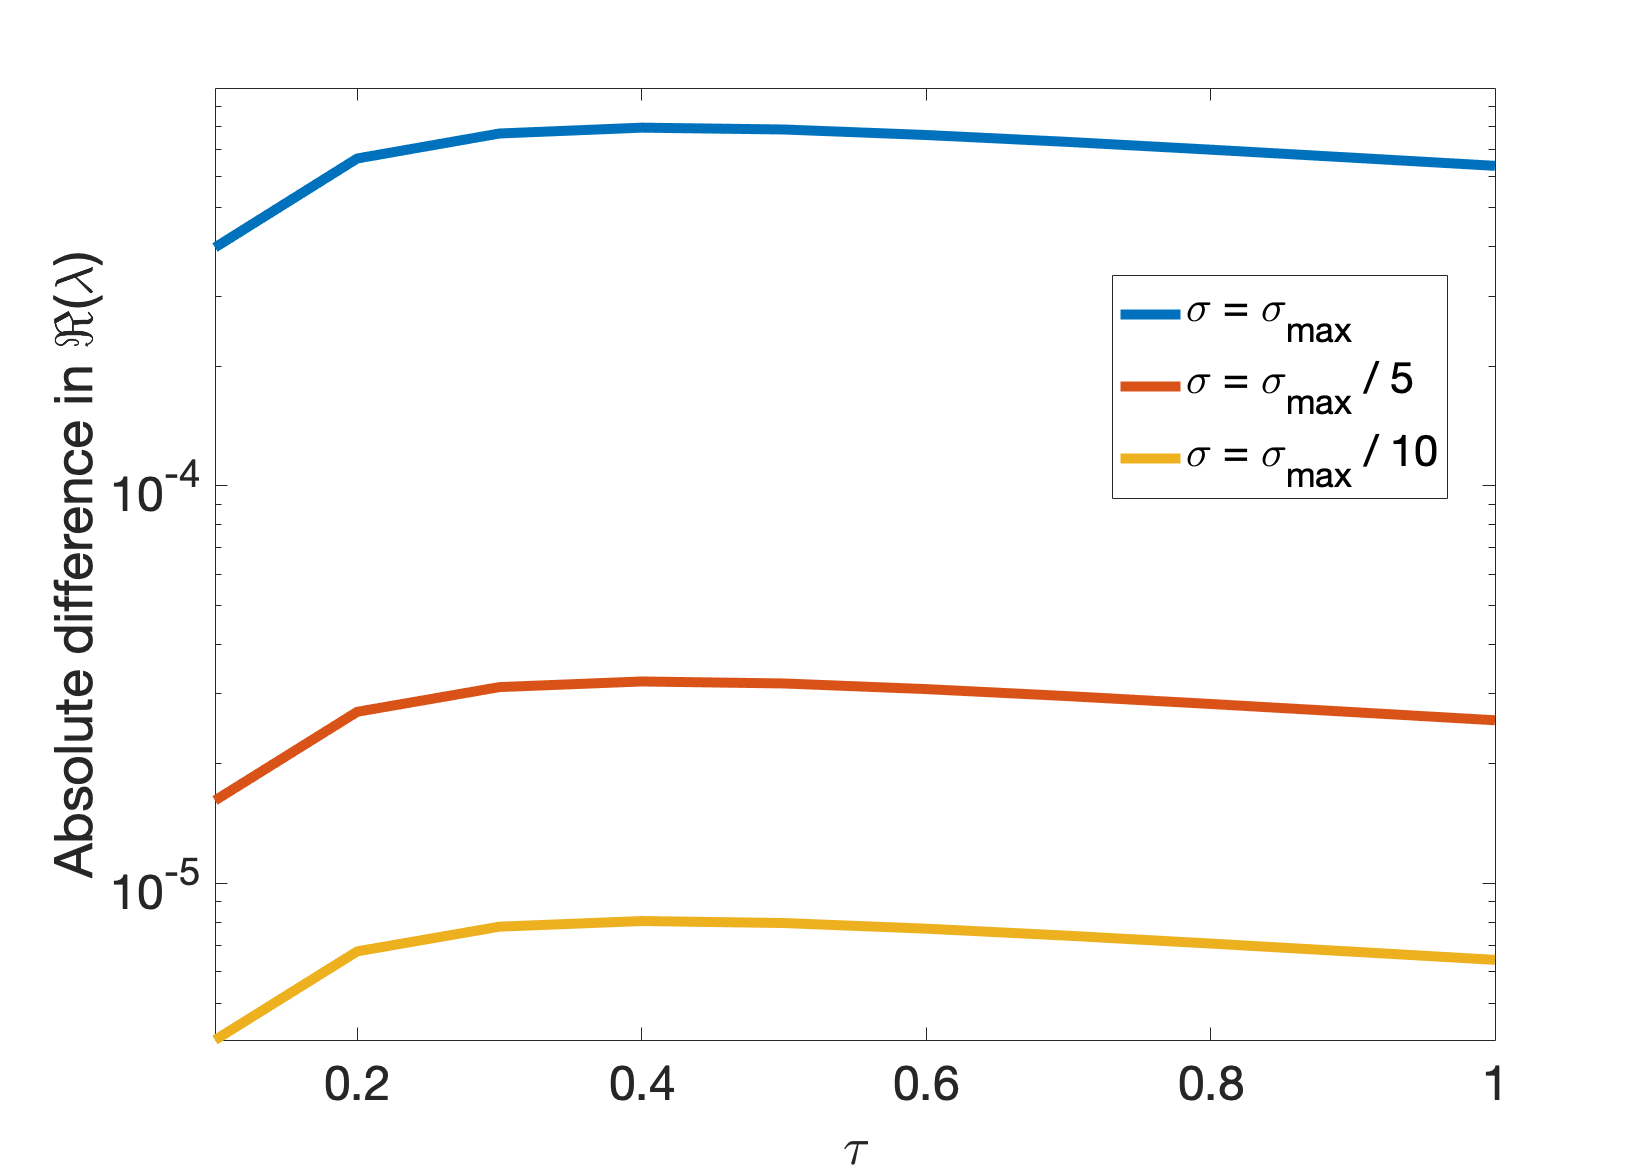
\includegraphics[width=7cm,height=5cm]{dispdiff1.png}
        \caption{Absolute difference in $\max_k(\Re(\lambda_k))$ as $\sigma$ is varied, between each distributed delay case and the fixed delay case.}
        \label{}
    \end{subfigure}
    \caption{$\max_k(\Re(\lambda_k))$ plotted against $\tau\in[0,1]$ for parameter set $(a,b)=(0.1,0.9)$. $\epsilon^2=0.001$ and $L=30\sqrt{0.05}$. $k$ is varied over $[0,50]$ at regular discrete intervals of $1$. Absolute difference of $\max_k(\Re(\lambda_k))$ between each of the distributed delay cases and fixed delay case plotted.}
    \label{fig:p2}
\end{figure}
% PARAMETER SET 3
\begin{figure}[H]
    \centering
    \begin{subfigure}[b]{0.45\textwidth}
        \centering
        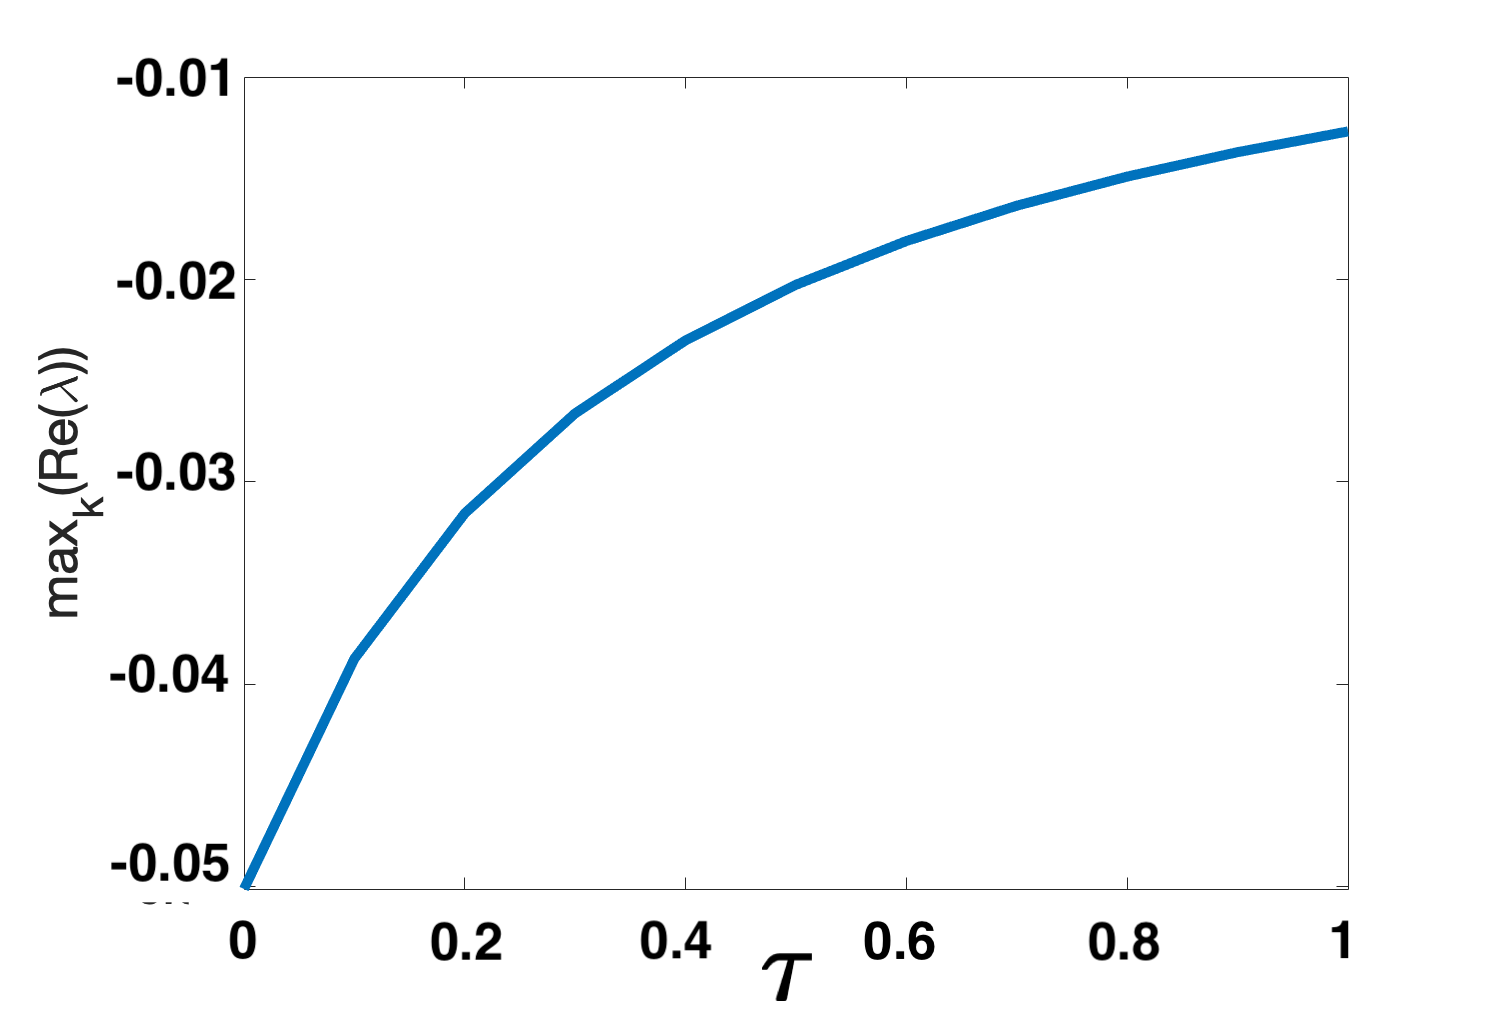
\includegraphics[width=7cm,height=5cm]{p3fixed.png}
        \caption{Fixed delay case.}
        \label{}
    \end{subfigure}
    \hfill
    \begin{subfigure}[b]{0.45\textwidth}
        \centering
        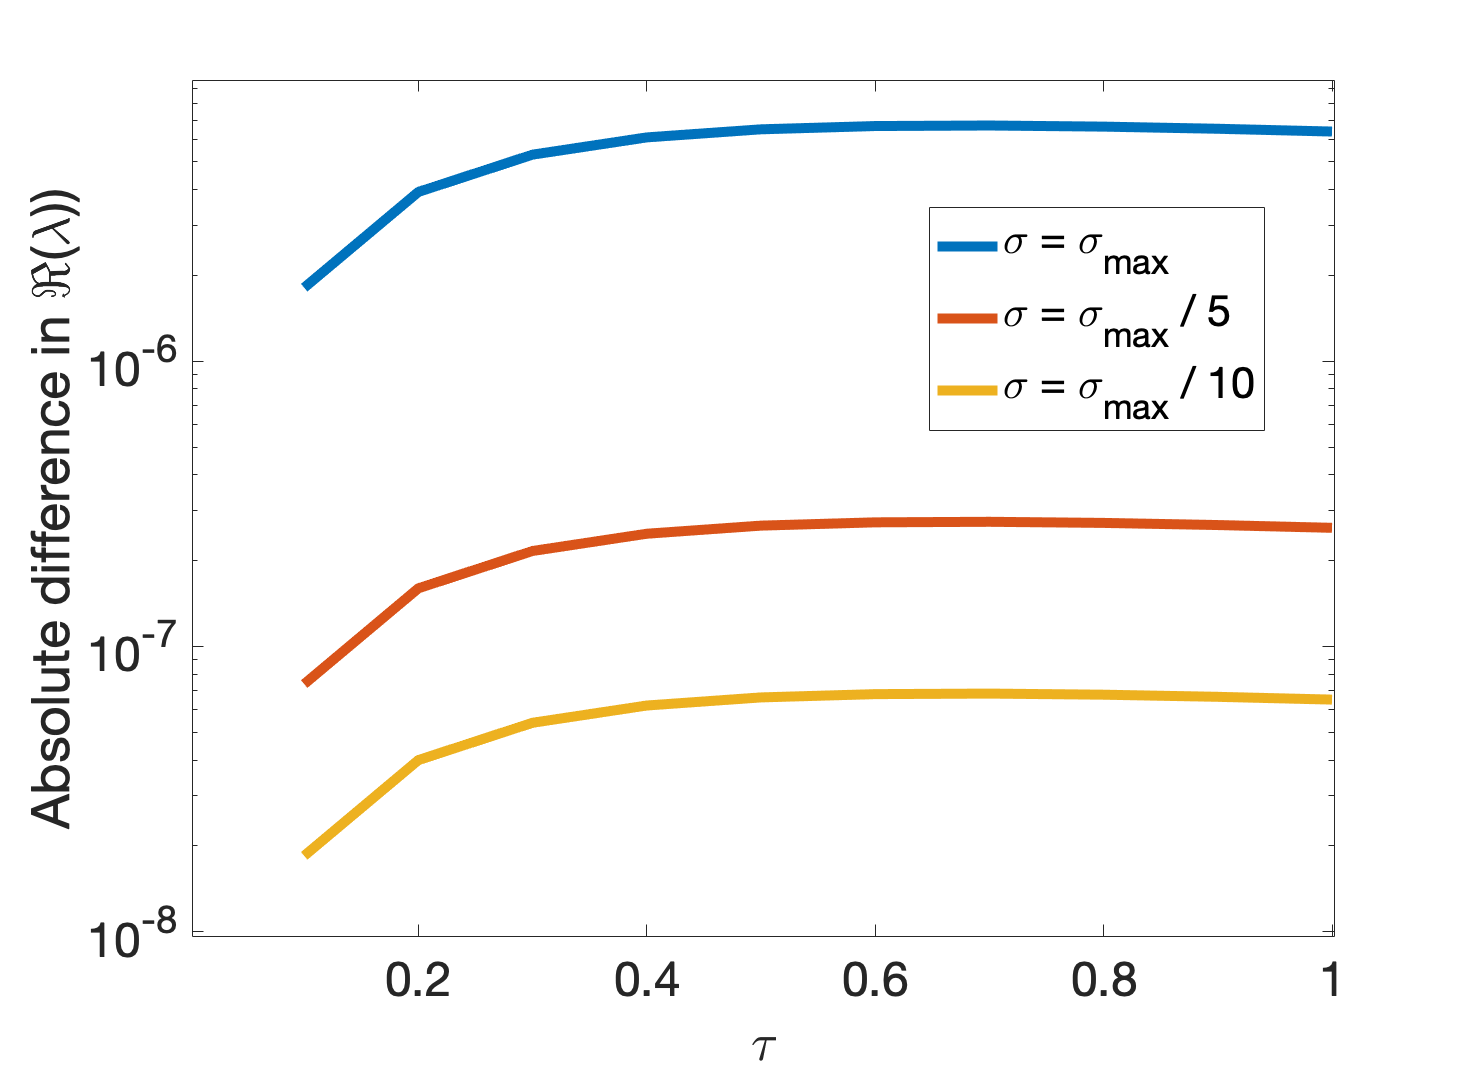
\includegraphics[width=7cm,height=5cm]{dispdiff2.png}
        \caption{Absolute difference in $\max_k(\Re(\lambda_k))$ as $\sigma$ is varied, between each distributed delay case and the fixed delay case.}
        \label{}
    \end{subfigure}
    \caption{$\max_k(\Re(\lambda_k))$ plotted against $\tau\in[0,1]$ for parameter set $(a,b)=(0.4,0.4)$. $\epsilon^2=0.001$ and $L=30\sqrt{0.05}$. $k$ is varied over $[0,50]$ at regular discrete intervals of $1$. Absolute difference of $\max_k(\Re(\lambda_k))$ between each of the distributed delay cases and fixed delay case plotted.}
    \label{fig:p3}
\end{figure}

Figures \ref{fig:p2} and \ref{fig:p3} show that, the largest variation in $\max_k(\Re(\lambda_k))$ when the largest $\sigma$ value is used. The results also suggest that for all $\sigma$ and $\tau\in[0,1]$ considered, that we expect to see pattern formation for $(a,b)=(0.1,0.9)$, but not for $(a,b)=(0.4,0.4)$. We note that that largest absolute difference in $\max_k(\Re(\lambda_k))$ across both parameter sets is of $O(10^{-5})$. This is an extremely small difference, on a similar order to numerical round off error, and is thus unlikely to make a qualitative difference on time-to-pattern. We verify these obvservations numerically in section \ref{section:distsim}.

 In order to consider how $\max_k(\Re(\lambda_k))$ varies across a larger parameter plane as $\sigma$ is varied, we consider the absolute difference of $\max_k(\Re(\lambda_k))$ for varying $\sigma$ values as a fraction of $\sigma_{max}$, for $\tau\in\{0.2,1\}$, against the fixed delay case. Figure \ref{fig:distheat} shows four different heatmaps of $\max_k(\Re(\lambda_k))$ across the parameter space for $\epsilon^2=0.001$ and fixed $\tau=0.2,1$. Overlayed onto these bifurcation plots are the contour lines at $\max_k(\Re(\lambda_k))=0$ and $\Re(\lambda_0)=0$, to highlight the Turing instability region. For each $(\tau,\epsilon^2)$, bifurcation plots were computed for the distributed delay case with varying $\sigma\in\{\sigma_{\max}\times0.99,\sigma_{\max}\times0.2,\sigma_{\max}\times0.1$. For each $(\tau,\epsilon^2)$, we consider the absolute difference of $\max_k(\Re(\lambda_k))$ between each distributed delay case and the fixed delay case, across the $(a,b)$ parameter space. These results are summarised in table \ref{tab:tab1}.
\begin{figure}[H]
    \centering
    \begin{subfigure}[b]{0.45\textwidth}
        \centering
        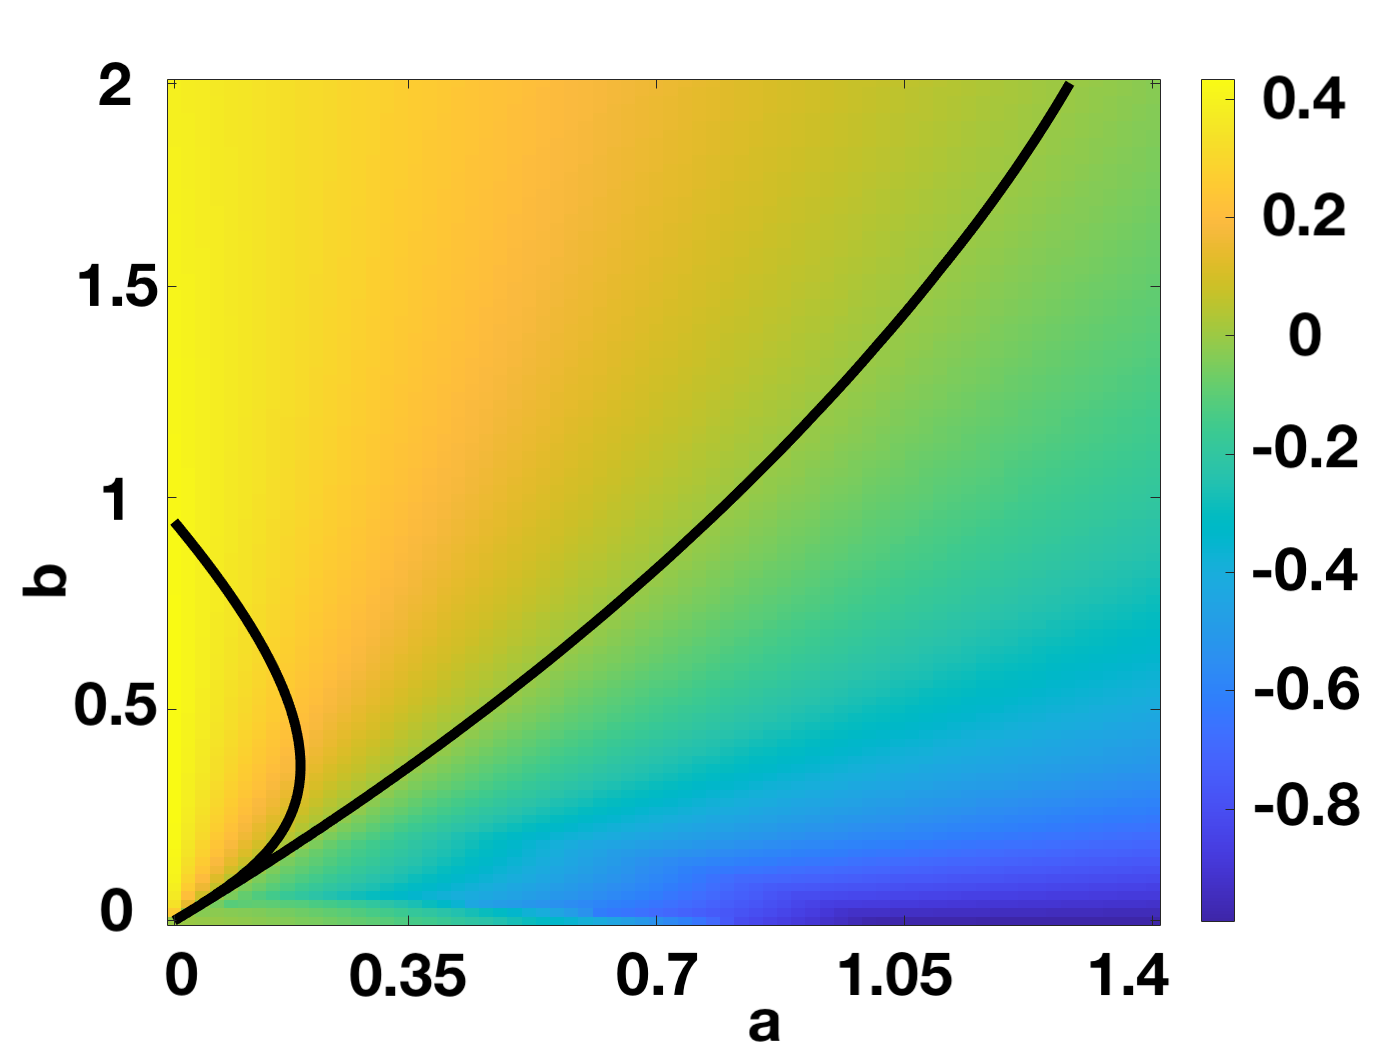
\includegraphics[width=7cm,height=4.75cm]{t1f1.png}
        \caption{$\tau=0.2$.}
        \label{}
    \end{subfigure}
    \hfill
    \begin{subfigure}[b]{0.45\textwidth}
        \centering
        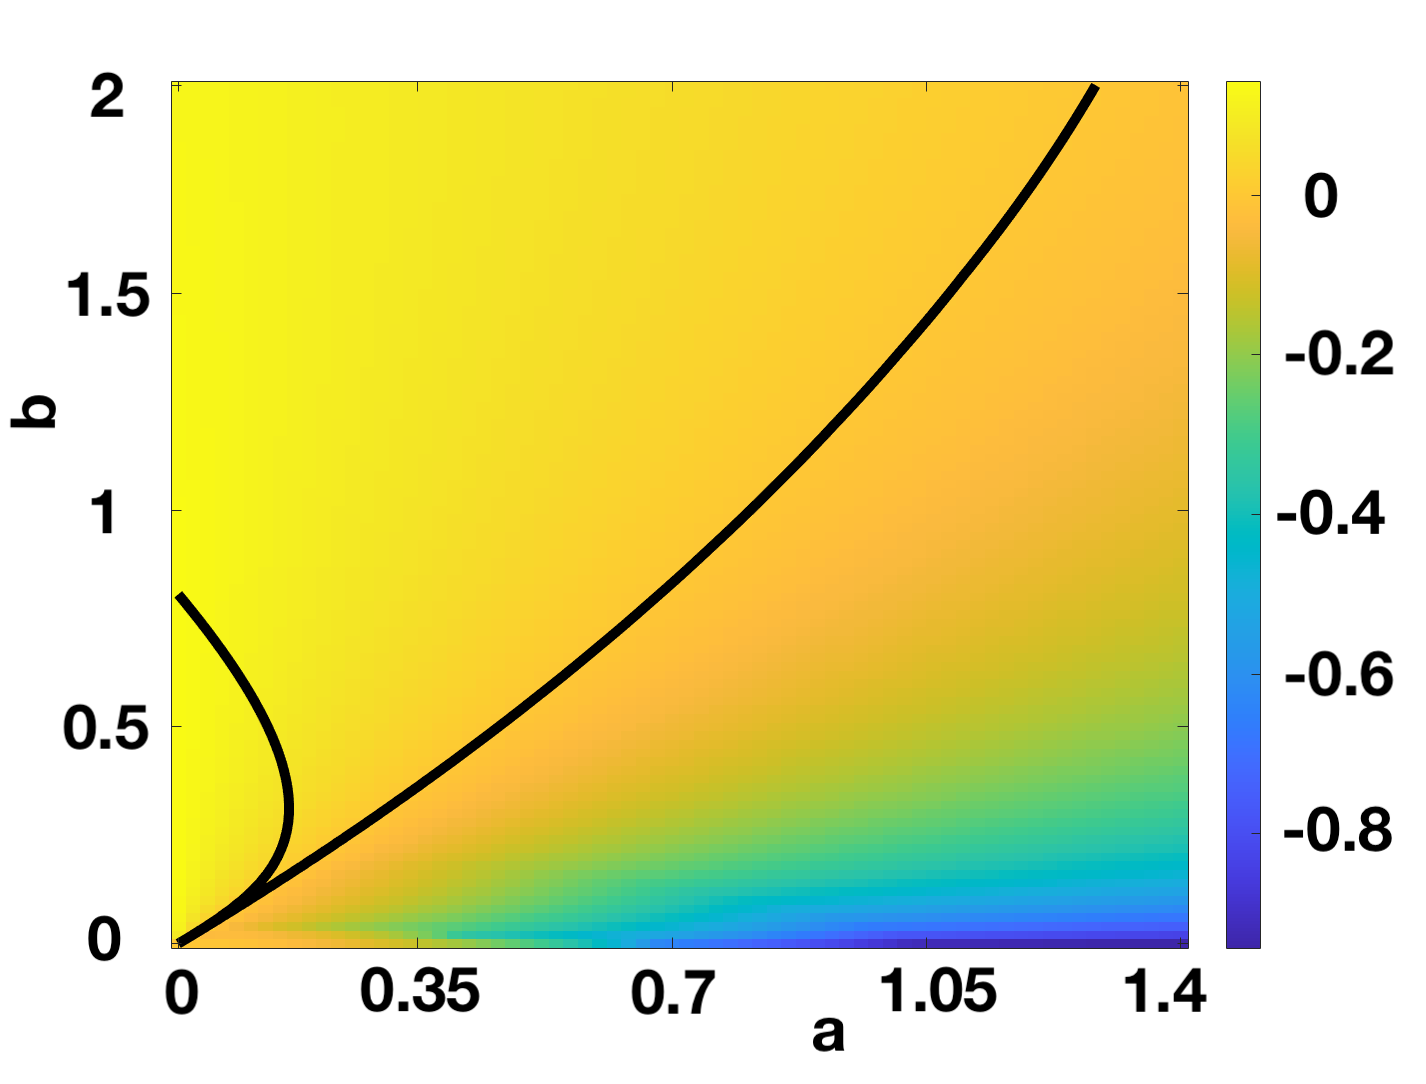
\includegraphics[width=7cm,height=4.75cm]{t2f1.png}
        \caption{$\tau=1$}
        \label{}
    \end{subfigure}
    \caption{Bifurcation diagrams produced by solving \eqref{characdist} for $\tau=0.2,1$ and $\epsilon^2=0.001$, on a domain length $L=30\sqrt{0.05}$.}
    \label{fig:distheat}
\end{figure}

We see that, for $\tau=0.2$, $|\max_k(\Re(\lambda_k))|$ is larger than that of $\tau=1$ across the parameter space. Observing the results in table \ref{tab:tab1}, the largest absolute difference in $\max_k(\Re(\lambda_k))$ for all $\sigma$ considered, and both $\tau=0.2,1$, across the parameter space $(a,b)\in[0,1.4]\times[0,2]$ is $O(10^{-3})$. We therefore expect that for all $(a,b)\in[0,1.4]\times[0,2]$,
using a symmetric Gaussian distribution centred at some mean $\tau$, for small $\tau$, will not significantly effect the time-taken until pattern formation compared to the fixed delay case, independent of the distribution. We numerically confirm these results for varying $\epsilon^2$, $\tau$ and $\sigma$, considering larger delays up to $\tau=8$, and differing $\epsilon^2$.

\begin{table}[]
\centering
\begin{tabular}{|l|c|l|l|l|}
\hline
\multicolumn{2}{|l|}{\multirow{2}{*}{}}                                                                                           & \multicolumn{3}{c|}{\textbf{$\sigma$}}                                                                                                                                    \\ \cline{3-5}
\multicolumn{2}{|l|}{}                                                                                                            & \multicolumn{1}{c|}{\textbf{$\sigma_{\max}\times0.99$}} & \multicolumn{1}{c|}{\textbf{$\sigma_{\max}\times0.2$}} & \multicolumn{1}{c|}{\textbf{$\sigma_{\max}\times0.1$}} \\ \hline
\multicolumn{1}{|c|}{\multirow{2}{*}{\textbf{\begin{tabular}[c]{@{}c@{}}Time \\ Delay ($\tau$)\end{tabular}}}} & \textbf{$0.2$} & $0.0010$                                                & $4.2\times10^{-5}$                                     & $1.1\times10^{-5}$                                     \\ \cline{2-5}
\multicolumn{1}{|c|}{}                                                                                           & \textbf{$1$}   & $0.0078$                                                 & $3.3\times10^{-4}$                                     & $8.2\times19^{-5}$                                     \\ \hline
\end{tabular}
\caption{Maximum, over $(a,b)$ parameter space, of absolute difference of $\max_k(\Re(\lambda_k))$ between each distributed delay case, for the given $\sigma$, and the fixed delay case, for each $\tau$. Parameters set as $\epsilon^2=0.001$ and $L=30\sqrt{0.05}$. All values given to 2.s.f. Due to numerical issues, results for the parameter range $b\in[1.9,2]$ were not considered.}
\label{tab:tab1}
\end{table}

\subsection{Numerical Results}\label{section:distsim}
Numerical simulations are shown here to verify the linear theory presented in section \ref{section:distlin}. We first confirm that the results obtained in figures \ref{fig:p2} and \ref{fig:p3} are accurate, namely that we find pattern formation for $(a,b)=(0.1,0.9)$ but not for $(a,b)=(0.4,0.4)$, independent of the $\tau\in[0,1]$ and $\sigma$ values considered. We also verify our main result, that modelling time delay as a symmetric Gaussian distribution will not quantitatively change the results seen from that of a fixed delay, independent of the $\sigma$ used. Figures \ref{fig:testdist1} and \ref{fig:testdist2} show the numerical solutions for $(a,b)=\{(0.1,0.9),(0.4,0.4)\}$ for $\tau=1$ and varying $\sigma$. Further numerical results with different $\tau$ and $\sigma$ values can be found in appendix \ref{section:appB}. Initial conditions were set as $\text{IC}_2$, as defined in \eqref{ICs}.

\begin{figure}[H]
    \centering
    \begin{subfigure}[b]{0.45\textwidth}
        \centering
        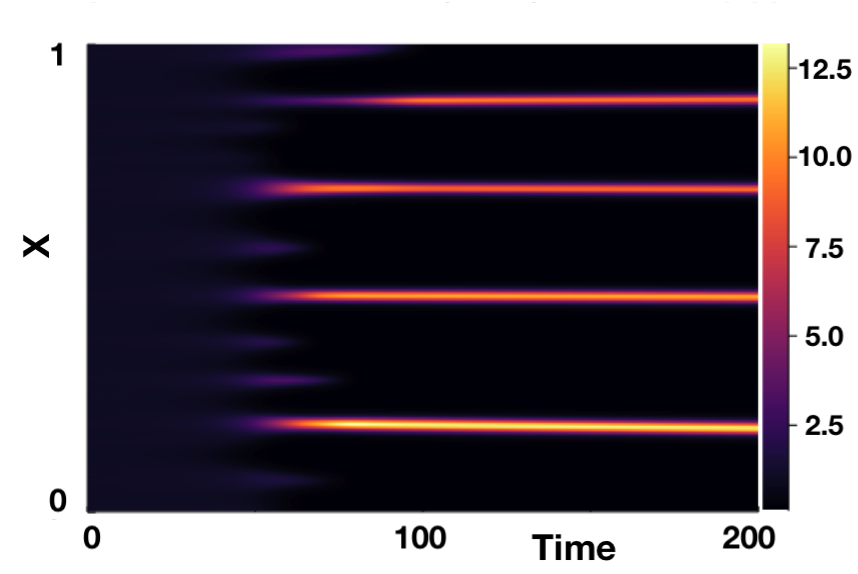
\includegraphics[width=7cm,height=5cm]{distp1sig1.png}
        \caption{Numerical solution with $\tau=1$ and $\sigma=\sigma_{max}\times0.99$.}
        \label{}
    \end{subfigure}
    \hfill
    \begin{subfigure}[b]{0.45\textwidth}
        \centering
        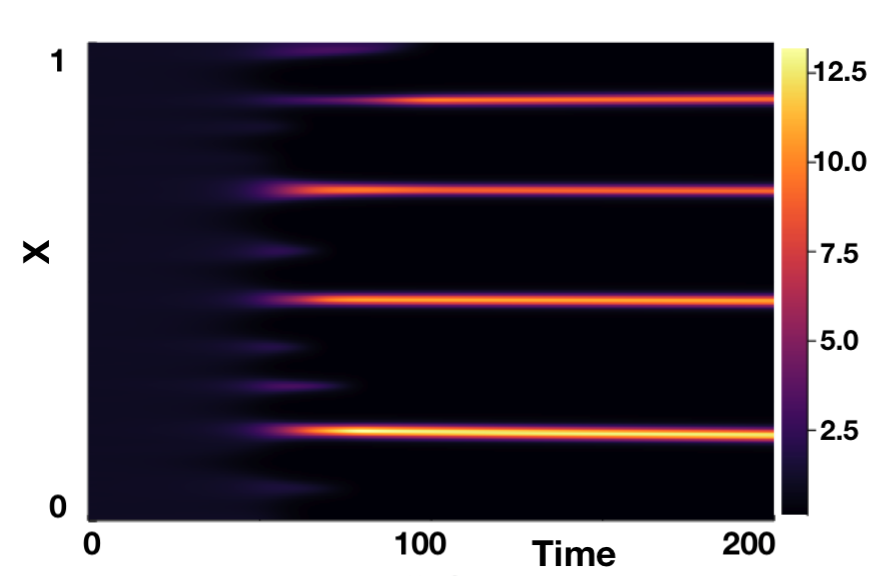
\includegraphics[width=7cm,height=5cm]{distp1sig2.png}
        \caption{Numerical solution with $\tau=1$ and $\sigma=\sigma_{max}\times0.1$.}
        \label{}
    \end{subfigure}
    \caption{Numerical solutions produced for $(a,b)=(0.1,0.9)$ with $\tau=1$ and $\sigma=\sigma_{max}\times0.99, \sigma_{max}\times0.1$. We use $L=30\sqrt{0.05}$ and $\epsilon^2=0.001$. $N=50$ quadrature points used for distributed delay.
    We see pattern formation, as predicted from linear theory.}
    \label{fig:testdist1}
\end{figure}

\begin{figure}[H]
    \centering
    \begin{subfigure}[b]{0.45\textwidth}
        \centering
        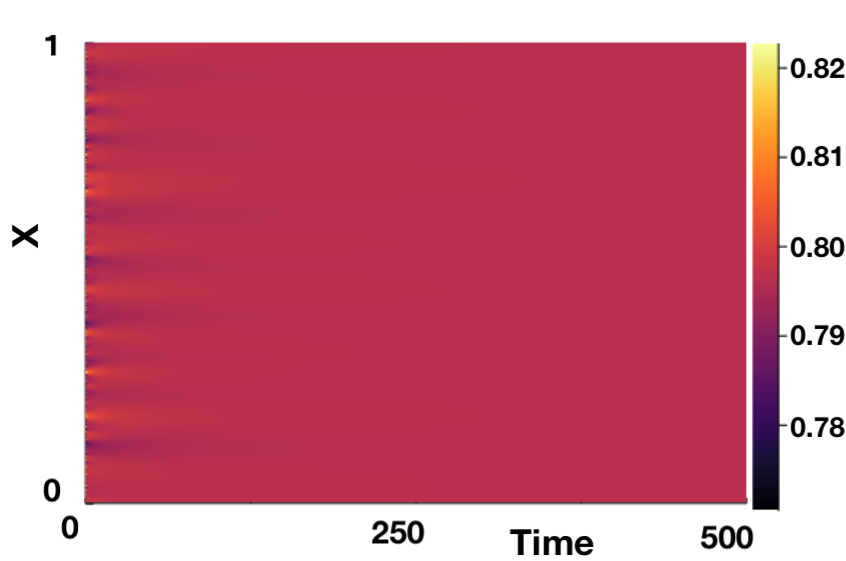
\includegraphics[width=7cm,height=5cm]{distp2sig1.png}
        \caption{Numerical solution with $\tau=1$ and $\sigma=\sigma_{max}\times0.99$.}
        \label{}
    \end{subfigure}
    \hfill
    \begin{subfigure}[b]{0.45\textwidth}
        \centering
        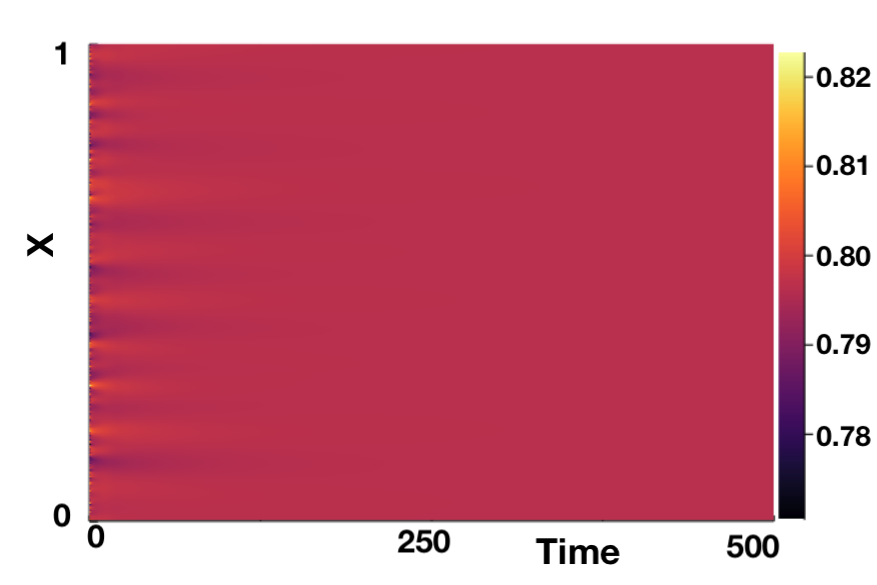
\includegraphics[width=7cm,height=5cm]{distp2sig2.png}
        \caption{Numerical solution with $\tau=1$ and $\sigma=\sigma_{max}\times0.1$.}
        \label{}
    \end{subfigure}
    \caption{Numerical solutions produced for $(a,b)=(0.4,0.4)$ with $\tau=1$ and $\sigma=\sigma_{max}\times0.99, \sigma_{max}\times0.1$. We use $L=30\sqrt{0.05}$ and $\epsilon^2=0.001$. $N=50$ quadrature points used for distributed delay. We see no pattern formation, as predicted from linear theory.}
    \label{fig:testdist2}
\end{figure}


\section{An Asymmetric Distribution}
\subsection{Introduction}
The results in section \ref{section:symmetric} suggest that using a symmetric Gaussian distribution does not have a quantitative effect on the results seen compared to that of the fixed delay case, and thus does not remedy the increased time-to-pattern problems caused by introducing a fixed time delay. We therefore consider how an asymmetric distribution, specifically a skewed truncated Gaussian distribution, affects the results compared to that of a fixed delay. Using the results in \cite{skewed}, the probability density function of the skewed truncated Gaussian distribution, $k(s;\mu,\omega,\rho)$, for some location $\mu$ and scaling $\omega$, is given by
\begin{equation}
    k(s;\mu,\omega,\rho)=\Psi_c\frac{2}{\sigma}f\left(\frac{s-\mu}{\omega}\right)\phi\left(\rho\frac{s-\mu}{\omega}\right),
\end{equation}
where the functions $f(x)$ and $\phi(x)$ are the same as those defined in \eqref{phi} and \eqref{f}. The new parameter $\rho$ is used to denote the scaling factor. The distribution is negatively skewed for $\rho>0$ and postively skewed for $\rho>0$. Finally, we have the $\Psi_c$ is the scaling constant for the truncation. This is given as
\begin{equation}
    \Psi_c=\frac{1}{F\left(\frac{b-\mu}{\omega},\rho\right)-F\left(\frac{a-\mu}{\omega},\rho\right)},
\end{equation}
with $F(x)$ the cdf of a skewed Gaussian distribution, described by
\begin{equation}
    F(x,\rho)=\phi(x)-2T(x,\rho).
\end{equation}
The function $T(x,\rho)$ denotes the Owen's T function \cite{owenst} and is written as an integral in the form
\begin{equation}
    T(x,\rho)=\frac{1}{2\pi}\int_0^\rho\frac{e^{-\frac{1}{2}x^2(1+s^2)}}{1+s^2}\ \text{d}s\quad -\infty<x,\rho<\infty.
\end{equation}
In the computational implementation of the skewed truncated Gaussian pdf, the integral $T(x,\rho)$ is resolved numerically using the composite Simpson's rule.

We note now that since the distribution is skewed, the parameters $\mu$ and $\omega$ no longer denote the mean and standard deviation of the distribution, but solely the location and scale of the distribution. To compare how the skewed distribution affects the onset of patterning compared to that of the fixed delay case, we require the mean of the skewed distribution, $\tau$, which is given by
\begin{equation}
    \tau=\int_a^bxk(x,\mu,\omega,\rho)\ \text{d}x.
\end{equation}
Using results from \cite{skewed}, the mean of the skewed truncated Gaussian distribution is computed as
\begin{equation}
\tau=\mu+\omega\Psi_c\left[k(a,\mu,\omega,\rho)-k(b,\mu,\omega,\rho)+\frac{2\rho}{\hat{\rho}\sqrt{2\pi}}\left(\phi\left(\hat{\rho}\frac{b-\mu}{\omega}\right)-\phi\left(\hat{\rho}\frac{a-\mu}{\omega}\right)\right)\right].
\end{equation}
The scalar $\hat{\rho}$ is given as $\hat{\rho}=\left(1+\rho^2\right)^{1/2}$.
